\section{STRIDE Modeling}

\begin{figure}[h!]
\centering
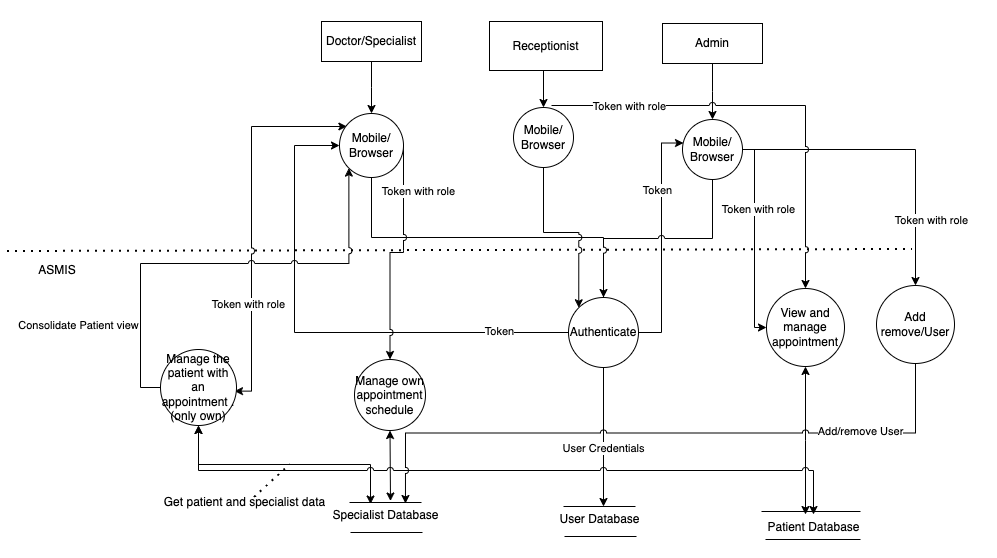
\includegraphics[width=\textwidth]{pics/dfd_staff.png}
\caption{DFD level 0 Staff for ASMIS}\label{fig:dfd_staff}
\end{figure}

\begin{figure}[h!]
\centering
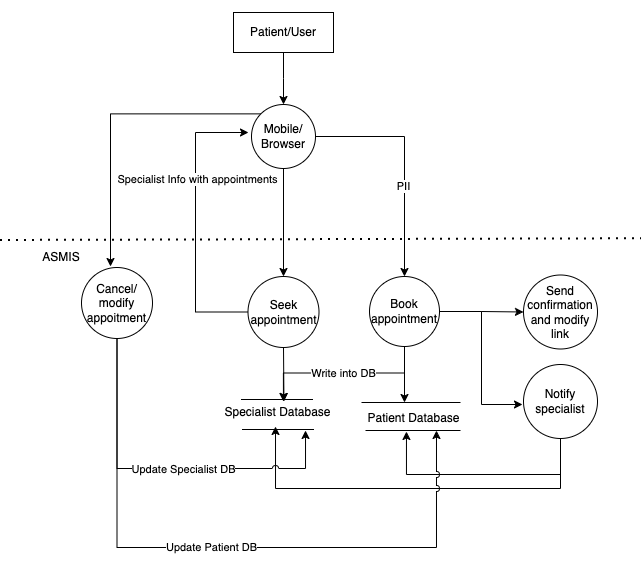
\includegraphics[width=12cm, height=11cm]{pics/dfd_user.png}
\caption{DFD level 0 User for ASMIS}\label{fig:dfd_user}
\end{figure}

\subsection{Overview}
STRIDE is one of the most mature threat analysis modeling methods. This method is adopted by Microsoft since 2002, where STRIDE just stands for a mnemonic, Spoofing, Tampering, Repudiation, Information disclosure, Denial of Service, and Elevation of privilege. Using these points it is also easier to discover and brainstorm possible threats. Its simplicity and its ability to find threats using dataflow diagrams made it a promising candidate for this report.\newline\newline
Figures \ref{fig:dfd_staff} and \ref{fig:dfd_user} depict the Level 0 dataflow diagram in respect to the different actors and how the system acts between the trusted boundaries. Additionally, from the DFD, we can identify the events and boundaries of the ASMIS system that would provide a concrete platform to perform STRIDE modeling \citep[p.~1]{shevchenko2018threat}.

\subsection{Spoofing}
